%%%%%%%%%%%%%%%%%%%%%%%%%%%%%%%%%%%%%%%%%%%%%%%%%%%%%%%%%%%%%%
%% LaTeX template for the science justification to be       %%
%%     submitted as part of a regular ALMA proposal.        %%
%% This template should also be used for a ToO, DDT, or     %%
%%     mm-VLBI ALMA proposal, but NOT for Large Programs    %%
%%     (these have a separate template with more sections)  %%
%%                                                          %%
%%                      ALMA Cycle 9                        %%
%%                                                          %%
%%%%%%%%%%%%%%%%%%%%%%%%%%%%%%%%%%%%%%%%%%%%%%%%%%%%%%%%%%%%%%

%%%%%%%%%%%%%%%%%%%%%%%%%%%%%%%%%%%%%%%%%%%%%%%%%%
%%%%% How to convert this document to PDF %%%%%%%%
%%%%%%%%%%%%%%%%%%%%%%%%%%%%%%%%%%%%%%%%%%%%%%%%%%

% If your figures are stored as PostScript files, you can use the 
% following commands to generate a PDF file of your proposal:

%% latex file.tex
%% dvips file.dvi
%% ps2pdf file.ps file.pdf 


% If your figures are PDF images or bitmap pictures in PNG, JPG, or GIF format,
% you can use the pdflatex command to generate a PDF file from this template
% (note, however, that the pdflatex command does not handle PostScript files):

% pdflatex file.tex

% Warnings: 
%           1. You must make sure that PDF output generated from this
%              template is complete both when displayed with a viewer 
%              (acroread, for example) and when printed on paper.
%              LaTeX installations vary greatly and therefore it might 
%              not be possible to get all proposals to come out 
%              correctly with a single text page layout. 
%              In some cases you will have to adjust the 
%              \topmargin=-7mm command in the template to center the 
%              text vertically in the page.  
%           2. The scientific justification, figures, tables, references,
%              and public outreach statement must all fit within the
%              4-page limit.
%           3. You are free to include colour images in your proposal justification.
%              Proposals are distributed to ALMA Review Panels and to distributed
%              peer review reviewers in electronic form.
%              However, the scientific content of the images should still remain
%              clear when displayed or printed in black and white.
%           4. This template is for regular, ToO, DDT, or mm-VLBI ALMA proposals,
%              but NOT for Large Programs: these have a separate template with
%              more sections, and is available from the ALMA Science Portal


%%%%%%%%%%%%%%%%%%%%%%%%%%%%%%%%%%%%%%%%%%%%%%
%%%%% Default format: 12pt single column %%%%%
%% 12pt is the minimum font size allowed !! %%
%% This applies to everything, including    %%
%% references, figure captions, and tables  %%
%% ==> Proposals not compliant to this will %%
%%     be rejected. See Section 5.3.1 in    %%
%%     the ALMA Proposer's Guide            %%
%%%%%%%%%%%%%%%%%%%%%%%%%%%%%%%%%%%%%%%%%%%%%%

\documentclass[12pt,a4paper]{article}  %% DO NOT CHANGE to 11pt or less !

\usepackage[dvipdfmx]{graphics, graphicx}
% if you on overleaf...
\usepackage{color}
% if you on local...
% \usepackage[dvipdfmx]{color}
\usepackage{amsmath,amssymb}
\usepackage{natbib}
\usepackage{aas_macros}
\usepackage{compactbib}
\usepackage{txfonts}
\usepackage{threeparttable}
\usepackage{xspace}
\usepackage{enumitem}
\usepackage{multicol}
\usepackage[rightcaption]{sidecap}
\usepackage[colorlinks=true,citecolor=blue]{hyperref}

\newcommand{\carbondioxide}{CO$_2$\xspace}
\newcommand{\protonatedcarbondioxide}{HCO$_2^+$\xspace}
\newcommand{\water}{H$_2$O\xspace}

%%%%%%%%%%%%%%%%%%%%%%%%%%%%
%%%%%% Page dimensions %%%%%
%%%%%%  DO NOT CHANGE  %%%%%
%%%%%%%%%%%%%%%%%%%%%%%%%%%%

\textheight=247mm
\textwidth=180mm
\topmargin=-7mm
\oddsidemargin=-10mm
\evensidemargin=-10mm
\parindent 10pt

%%%%%%%%%%%%%%%%%%%%%%%%%%%%%
%%%%% Start of document %%%%% 
%%%%%%%%%%%%%%%%%%%%%%%%%%%%%

\begin{document}
\pagestyle{plain}
\pagenumbering{arabic}
 
% The title, abstract and list of investigators should NOT be included in the
% Scientific justification. The title and abstract are put automatically on the cover page.

%%%%%%%%%%%%%%%%%%%%%%%%%%%%%%%%%%%%%%%%%
%%%%% Body of science justification %%%%%
%%%%%%%%%%%%%%%%%%%%%%%%%%%%%%%%%%%%%%%%%

%% ENTER TEXT, FIGURES AND TABLES BELOW
%% Minimum font size for all text, references, figure captions, and tables is 12pt
%% Proposals not compliant to this will be rejected. See Section 5.3.1 in the ALMA Proposer's Guide.

\section{Scientific justification}

\subsection{Background}

Carbon dioxide (\carbondioxide) is an abundant species in interstellar ice and one of the dominant carriers of oxygen and carbon in the interstellar medium (ISM). \carbondioxide is abundant in cometary ices and planetary atmospheres as well. To understand how \carbondioxide in the ISM will be incorporated into planetary systems, it is essential to reveal its abundance and distribution in planet-forming regions. More specifically, locating the \carbondioxide snowline (i.e., sublimation front, $\sim$50\,K) in the protostellar envelopes or disks is crucial as it will constrain the distributions of \carbondioxide in gas and solid phases. The location of the \carbondioxide snowline is also closely related to planet formation as the poorer stickiness of \carbondioxide ices may inhibit the growth of dust grains \citep[e.g.,][]{Okuzumi19}. Recent observational studies showing substructures possibly caused by the grain growth in protostellar objects \citep[e.g.,][]{Sheehan20, Ohashi21} have made it even more important to probe the \carbondioxide snowline location in those young sources to understand the origin of those substructures.


% Recent observational studies suggesting grain growth or potential planet formation in young protostellar objects \citep[e.g.,][]{Sheehan20, Ohashi21} have made it even more important to probe the \carbondioxide snowline location in those young sources.

However, as the direct observations of gas phase \carbondioxide are challenging, the distributions of \carbondioxide in the protostellar envelopes and disks are still poorly understood. The solid phase \carbondioxide has been widely observed in infrared absorption bands, and its abundance has been estimated to be $\sim$15--50\% with respect to \water ice around low-mass protostars \citep{Oberg11}. On the other hand, due to the lack of permanent dipole moment, gas phase \carbondioxide is observable only with ro-vibrational absorption or emission in infrared. The high dust opacity and low spatial resolution of infrared observations make it difficult to explore the distribution of gas phase \carbondioxide (or the location of \carbondioxide snowline) toward protostars deeply embedded in the dusty envelopes. \textbf{Here, we propose to instead observe the protonated carbon dioxide (\protonatedcarbondioxide), the gas phase \carbondioxide tracer, at high angular resolutions with ALMA to observationally locate the \carbondioxide snowline in protostellar envelopes for the first time. This will be a crucial first step to understanding the \carbondioxide chemistry as well as its role in planet formation in protostellar objects.}

\subsection{Protonated carbon dioxide as a gas phase \carbondioxide tracer}
Protonated carbon dioxide, \protonatedcarbondioxide (or HOCO$^+$), is considered to be a good tracer of gas phase \carbondioxide because its abundance and distribution are directly related to those of gas phase \carbondioxide \citep[e.g.,][]{Sakai08}. Figure \ref{fig:protocore_cartoon} shows the schematic illustration of the protostar, protostellar disk, and protostellar envelopes. As Figure \ref{fig:protocore_cartoon}(a) illustrates, outside the \carbondioxide snowline, where the temperature is $\lesssim$50\,K (i.e., cold or lukewarm envelope), \carbondioxide is mainly formed in the solid phase, e.g., CO + H $\longrightarrow$ HCO and HCO + O $\longrightarrow$ \carbondioxide + H. In this regime, \protonatedcarbondioxide is mainly formed via HCO$^+$ + OH $\longrightarrow$ \protonatedcarbondioxide + H with much less contribution from \carbondioxide + H$_3^+$ as \carbondioxide is locked into ice. Once the \carbondioxide sublimates at the snowline ($\sim$50\,K), the gas phase abundance of \carbondioxide rapidly increases and the dominant formation pathway of \protonatedcarbondioxide will be \carbondioxide + H$_3^+$ $\longrightarrow$ \protonatedcarbondioxide + H$_2$, which will increase the \protonatedcarbondioxide abundance as well. 
% The formation of \protonatedcarbondioxide is balanced with the destruction via CO + \protonatedcarbondioxide $\longrightarrow$ \carbondioxide + HCO$^+$. 
Finally, inside the \water snowline ($\gtrsim$100\,K, i.e., warm inner envelope or disk), the \protonatedcarbondioxide abundance will rapidly decrease due to the destruction by \water. In short, \textbf{the spatial distribution of \protonatedcarbondioxide is expected to be ring-shaped; the outer and inner edge of the ring corresponds to the \carbondioxide and \water snowline, respectively. Thus, \protonatedcarbondioxide is expected to be a good tracer of the \carbondioxide sublimation region.} 

The astrochemical model with detailed physical structures of protostellar envelopes has supported this picture. Figure \ref{fig:protocore_cartoon}(b) presents the distributions of related molecules as a function of temperature, calculated based on the methods presented in \citet{Aikawa20}. Indeed, the \protonatedcarbondioxide abundance increases at $\sim$50\,K along with the sublimation of \carbondioxide, and then rapidly decreases at $\sim$100\,K at the \water snowline. Related molecules also show interesting behavior. C$_2$H and HCO$^{+}$ abundances decrease at \carbondioxide snowline and further at \water snowline, which might be complementary tracers of \carbondioxide sublimation.  

\protonatedcarbondioxide has previously been detected in the cold ($\sim$10\,K) outer envelopes of several low-mass protostars \citep[e.g.,][]{Sakai08, Vastel16, Majumdar18}. However, all of the detection has been reported with single-dish observations, and therefore the distributions of \protonatedcarbondioxide in the \carbondioxide sublimation region have never been mapped.

\begin{figure}[th]
    \centering
    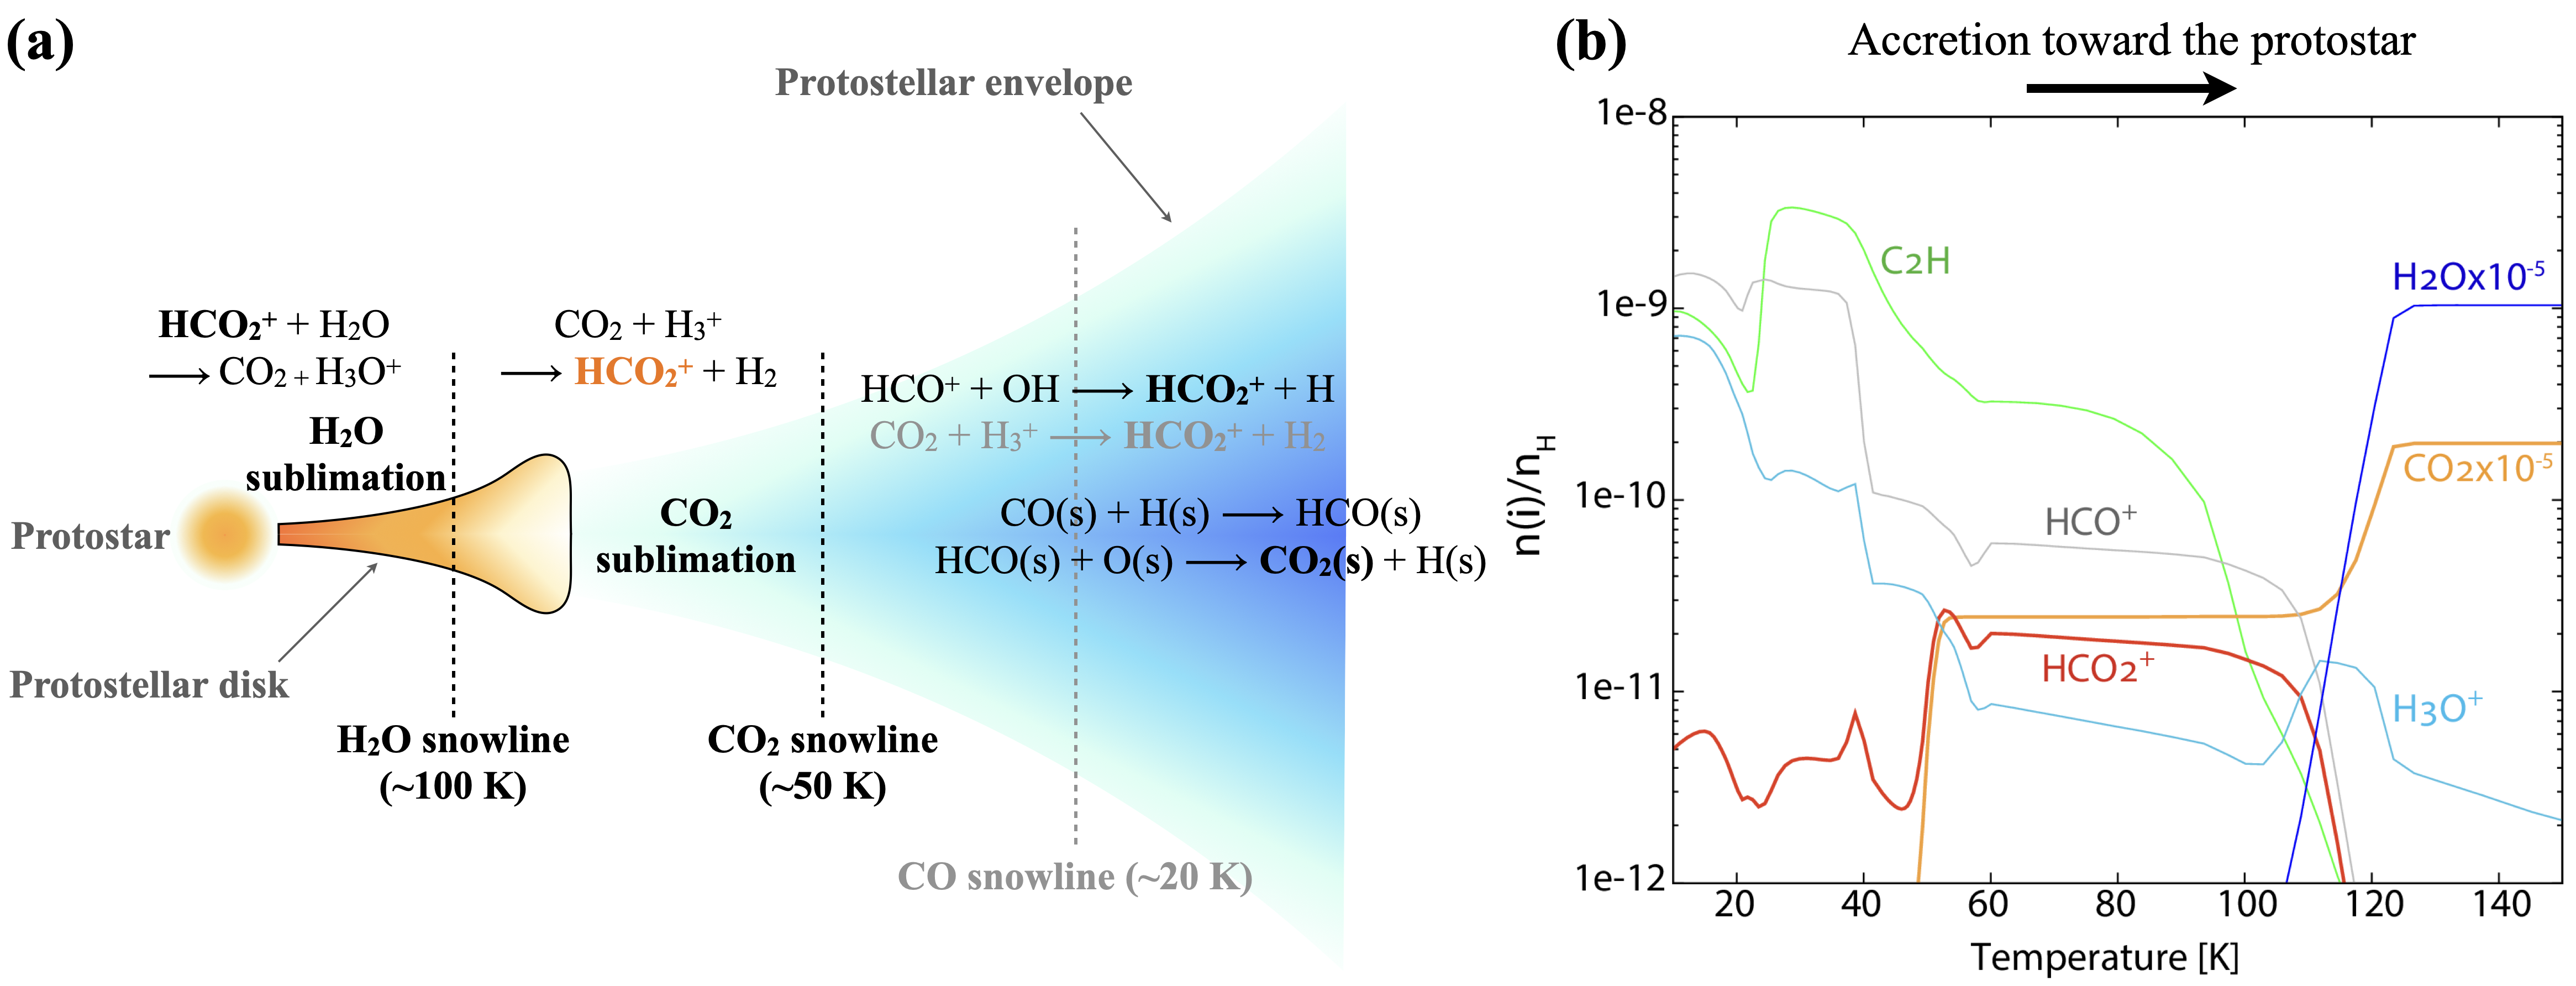
\includegraphics[width=\textwidth]{protostellar_core_HCO2p_cartoon_model.png}
    \caption{\em{(a) Illustration of the cross section of a protostellar core and formation pathways of \protonatedcarbondioxide in each region. (s) denotes the solid phase reactions. The abundance of \protonatedcarbondioxide will increase between the \carbondioxide snowline and \water snowline. (b) The abundance of related species in the protostellar core model based on \citet{Aikawa20} as a function of temperature. The \protonatedcarbondioxide abundance increases between $\sim$50\,K and $\sim$100\,K.}}
    \label{fig:protocore_cartoon}
\end{figure}
\vspace{-2em}

\subsection{Proposed observations}
We propose to observe the multiple lines of \protonatedcarbondioxide in Band 3 and 6 toward the protostellar source L483 at 0\farcs28--0\farcs5 resolution. Our immediate objectives are:

\vspace{-0.5em}
\begin{enumerate}[leftmargin=*]
    \setlength\itemsep{-0.2em}
    
    \item[1.] \textbf{Measuring the location of the \carbondioxide snowline} by spatially resolving the \protonatedcarbondioxide line emission. This requires a sufficient angular resolution of 0\farcs28--0\farcs5 (or $\sim$60--100\,au), assuming the distance of 200\,pc.
    \item[2.] \textbf{Constraining the abundance distributions of \carbondioxide} by comparing the observed \protonatedcarbondioxide abundance to the protostellar core models. This requires multiple lines of \protonatedcarbondioxide and a combination of astrochemical models with detailed physical structures.
    % measuring the distributions of \protonatedcarbondioxide column density and excitation temperature. This requires multiple lines of \protonatedcarbondioxide and well-established chemical scheme to estimate the \carbondioxide abundance from \protonatedcarbondioxide.
\end{enumerate}
\vspace{-0.5em}

\noindent \textbf{Target sources and lines} \quad The proposed target L483 is a well-known, nearby ($\sim$200\,pc) Class 0 protostellar core that shows both warm carbon chain chemistry (WCCC) and hot corino chemistry \citep[Figure \ref{fig:prev_obs},][]{Oya17}: while in the outer region ($\sim$a few hundred au, $\lesssim$50\,K) emission from unsaturated hydrocarbons such as C$_4$H and C$_2$H widely appears with possible inner cavities, several lines of water isotopologues and complex organic molecules (COMs) such as CH$_3$OH have been detected in the innermost warm region \citep[$\lesssim$100\,au, $\gtrsim$100\,K, see also][]{Jensen19, Jensen21}, showing the sequential sublimation of icy molecules with different sublimation temperatures due to the increase of temperature toward the central region, which is the similar situation to the model in Figure \ref{fig:protocore_cartoon}(b). Since \carbondioxide has a sublimation temperature of $\sim$50\,K, similar to CH$_4$ (the feedstock of carbon chain molecules), the previous detection of carbon chain molecules makes this source an ideal test-bed for constraining the \carbondioxide snowline. In addition, the physical and chemical characteristics of the source have been well studied, which makes the interpretation of proposed observations straightforward. \citet{Jacobsen19} observed several molecular lines in Band 7 at $\sim$0\farcs1 (or $\sim$20\,au) resolution. HCO$^+$ ($J=$ 4--3) presents a complicated emission morphology, suggesting that the estimates of \carbondioxide snowline with this line is difficult. The COMs lines show a quite compact (but marginally spatially resolved) emission from the inner $\sim$40\,au, implying the inner hot region where water and COMs have sublimated. They also estimated the dust temperature distribution from dust continuum observations, indicating the \carbondioxide sublimation at $\sim$180\,au (where the dust temperature becomes $\sim$50\,K).  Finally and most importantly, the previous detection of solid \carbondioxide (\carbondioxide/\water $\sim$ 44\%) in infrared observations \citep{Boogert11} and \protonatedcarbondioxide with single-dish radio observations \citep{Agundez19} makes L483 a promising protostellar source to detect \protonatedcarbondioxide. %\citet{Boogert11} revealed a significant amount of solid \carbondioxide (\carbondioxide/\water $\sim$ 44 per cent) in infrared absorption observations, implying that there is also a large amount of sublimated \carbondioxide gas. 
The \protonatedcarbondioxide abundance in the cold outer envelope has been estimated to be $\sim7\times10^{-12}$ with a temperature of 10\,K, which is similar to the value at 10\,K in the model presented in Figure \ref{fig:protocore_cartoon}(b).%As B335 has the similar physical and chemical structure, detection toward B335 is promising as well.  

We propose to observe multiple lines of \protonatedcarbondioxide with different excitation energies in Band 3 and 6, which enables us to conduct the excitation analysis. The combination of Band 3 and Band 6 provides unique access to 6 lines with a wide range of excitation energies (10--120\,K), which is essential to determine the excitation temperature and column density of \protonatedcarbondioxide simultaneously. 
% Excitation temperature is a good proxy of the gas temperature of the molecule in LTE condition, and thus used to confirm that observed \protonatedcarbondioxide emission probe the sublimation of \carbondioxide ($\sim$50\,K). Column density of \protonatedcarbondioxide is directly used to infer the abundance of \carbondioxide (using a simplified chemical scheme, see below).

\smallskip
\noindent \textbf{Analysis method and impact} \quad First, we will directly estimate the snowline location by the spatially resolved image of \protonatedcarbondioxide lines (Goal 1). Additional lines of HCO$^+$ isotopologues and C$_2$H will be complementarily used to confirm the \carbondioxide snowline location. As the abundances of these molecules would decrease along with \carbondioxide sublimation (Figure \ref{fig:protocore_cartoon}b), these lines would show the spatially anti-correlated distributions against \protonatedcarbondioxide lines. In addition, the \protonatedcarbondioxide emission will show an inner cavity that corresponds to the water sublimation region (Figure \ref{fig:protocore_cartoon}(b)). This can be compared to the additional HDO line in Band 6. The combination of these lines will completely reveal the \carbondioxide sublimation region as schematically illustrated in Figure \ref{fig:prev_obs}(b). The excitation temperature derived from the multi-line analysis is also useful to confirm that observed \protonatedcarbondioxide emission probes the sublimation of \carbondioxide ($\sim$50--100\,K).

Second, we will conduct the excitation analysis using multiple lines of \protonatedcarbondioxide (i.e., rotation diagram method) to derive the column density distributions of \protonatedcarbondioxide, and then constrain the distributions of the \carbondioxide abundance using detailed physical/chemical models (Goal 2). The \protonatedcarbondioxide abundance is mostly determined by a balance between the formation (H$_3^+$ + \carbondioxide) and destruction (\protonatedcarbondioxide + CO), from which we will obtain a precise constraint on the \carbondioxide abundance distribution. This chemical scheme depends on the ionization rate and gas density: we can obtain the estimates of ionization rate from complementary HCO$^+$ observations and that of gas density from detailed physical models \citep[e.g.,][]{Aikawa20} and extensive previous observations \citep[e.g.,][]{Jacobsen19}, which will further improve the accuracy of \carbondioxide abundance estimates.   


% Since \protonatedcarbondioxide abundance is sensitive to the gas phase \carbondioxide abundance, we will obtain a precise constraint on it.  

These estimates on the location of the \carbondioxide snowline and abundance distributions of \carbondioxide have significant impacts on astrochemistry. We will use these results to \textbf{benchmark the existing astrochemical protostellar core model}, \textbf{interpret how \carbondioxide will be incorporated into planet-forming disks and eventually the planetary systems}, and \textbf{understand possible grain growth or planet formation in young protostellar disks}. The proposed observations will also provide a useful benchmark for future \protonatedcarbondioxide line observations of other protostellar sources. 

\vspace{-1em}
\begin{figure}[th]
    \centering
    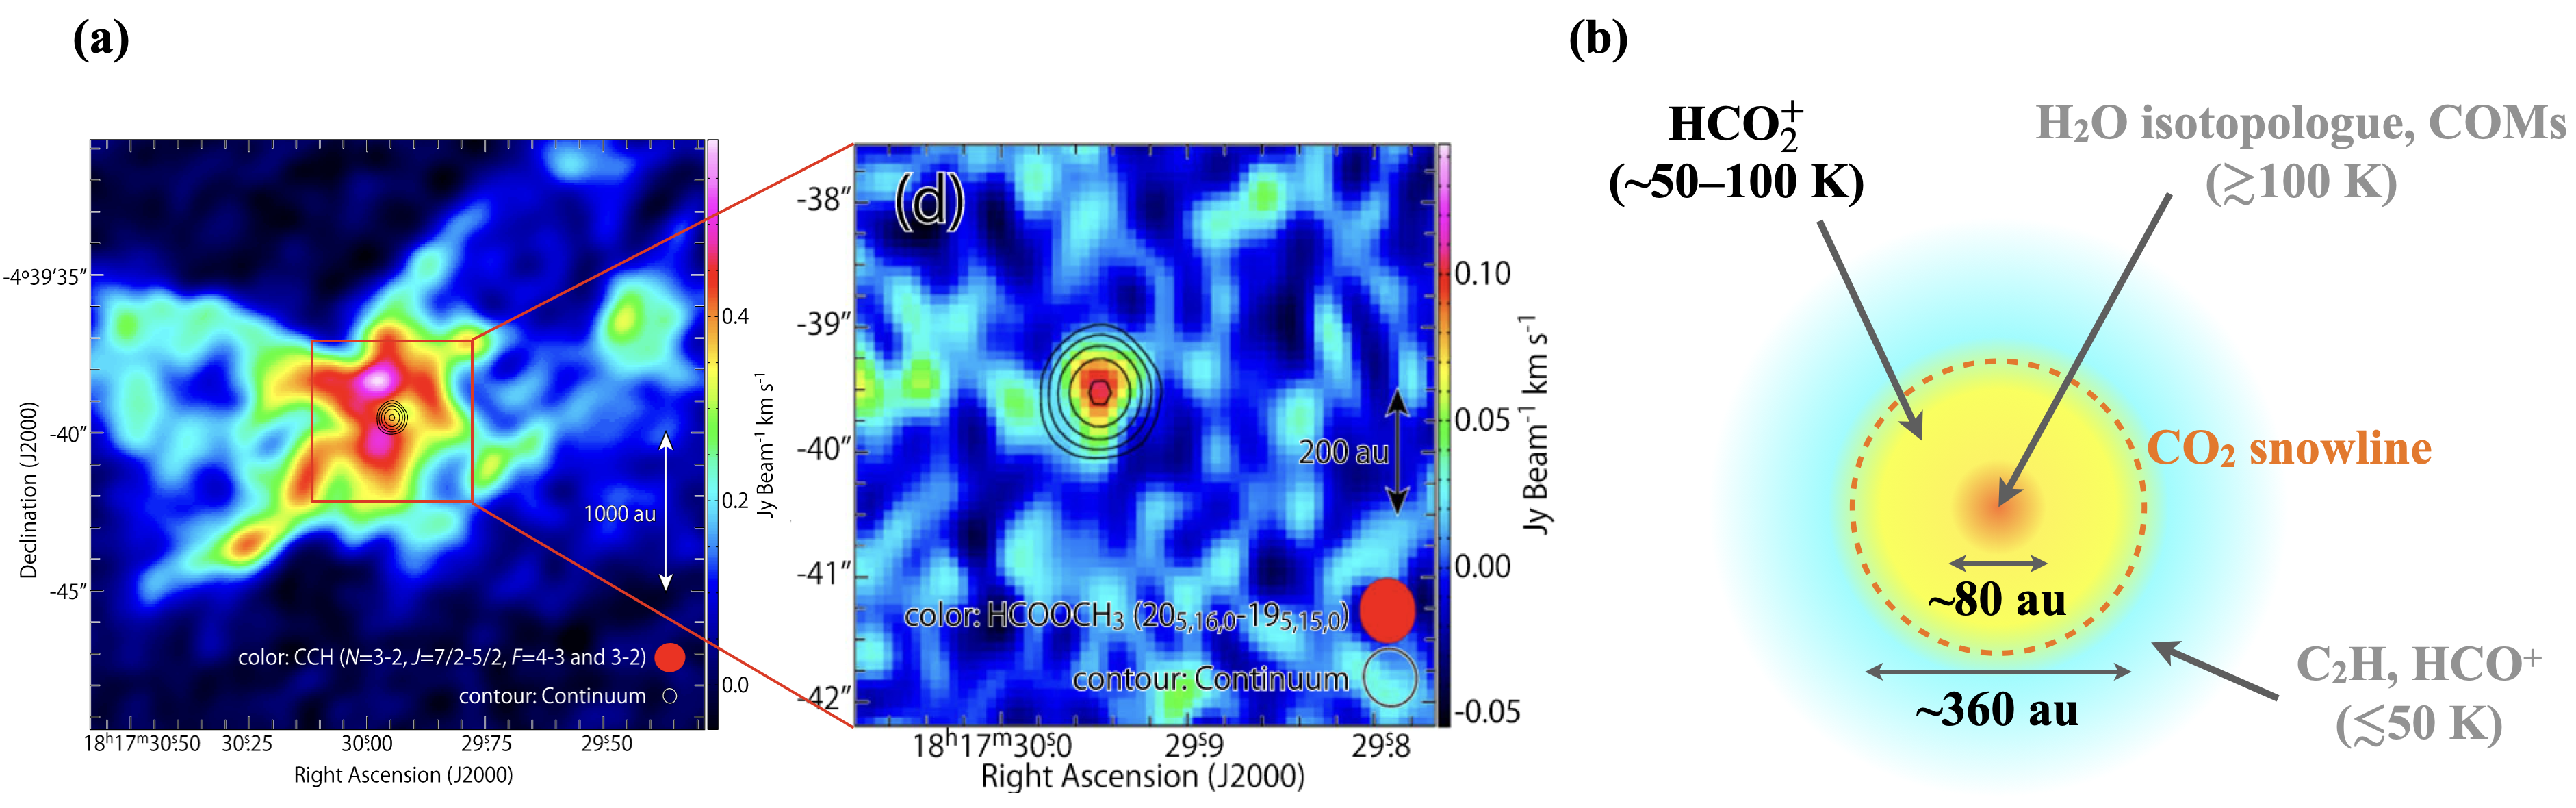
\includegraphics[width=\textwidth]{L483_prevobs_cartoon.png}
    \caption{\emph{(a) Previous observations of the carbon chain molecule (C$_2$H) and complex organic molecule (HCOOCH$_3$) toward L483 \citep{Oya17}. While C$_2$H shows the extended emission, HCOOCH$_3$ presents compact emission in the innermost region. Note that the scales of the two panels are different. (b) Schematic illustrations of expected distributions of molecules. Note that the emitting region sizes are not scaled.}}
    \label{fig:prev_obs}
\end{figure}


% ALMA uses two systems to review the proposals submitted in the Main Call.
% All proposals requesting less than 50 h on the 12-m Array and all ACA stand-alone proposals requesting less
% than 150 h on the 7-m Array will be reviewed by Distributed peer review (see Section 1.2.1 of the Proposer's Guide).
% All Large Programs will be reviewed by Panels. 
% Additionally, both systems will follow a dual-anonymous procedure, in which the proposers do not know
% who are the reviewers and the reviews do not who are the proposers.
%
% Please refer to the guidelines before writing your proposal:
%     https://almascience.org/proposing/alma-proposal-review/dual-anonymous
%
% In the following part, describe the scientific background of the project,
% pertinent references and previous work relevant to this 
% proposal, together with any figures and tables that you judge necessary
% (use the following two examples as templates, or remove)
% Please do not disclose the name(s) of the proposer(s), and write the proposal in a way
% such that the proposer(s) cannot be identified. 
 
%-----------------------------Figure Start---------------------------

% The 'scale' parameter below allows you to scale the figure so that it fits within the page.
% In this case the figure was scaled to 20% of its original size.
% Note: for .png files one has to use pdflatex, not classic latex
%
% Minimum font size for references: 12pt 
% Proposals not compliant to this will be rejected. See Section 5.3.1 in the ALMA Proposer's Guide.

% \begin{figure}[tbh]
% 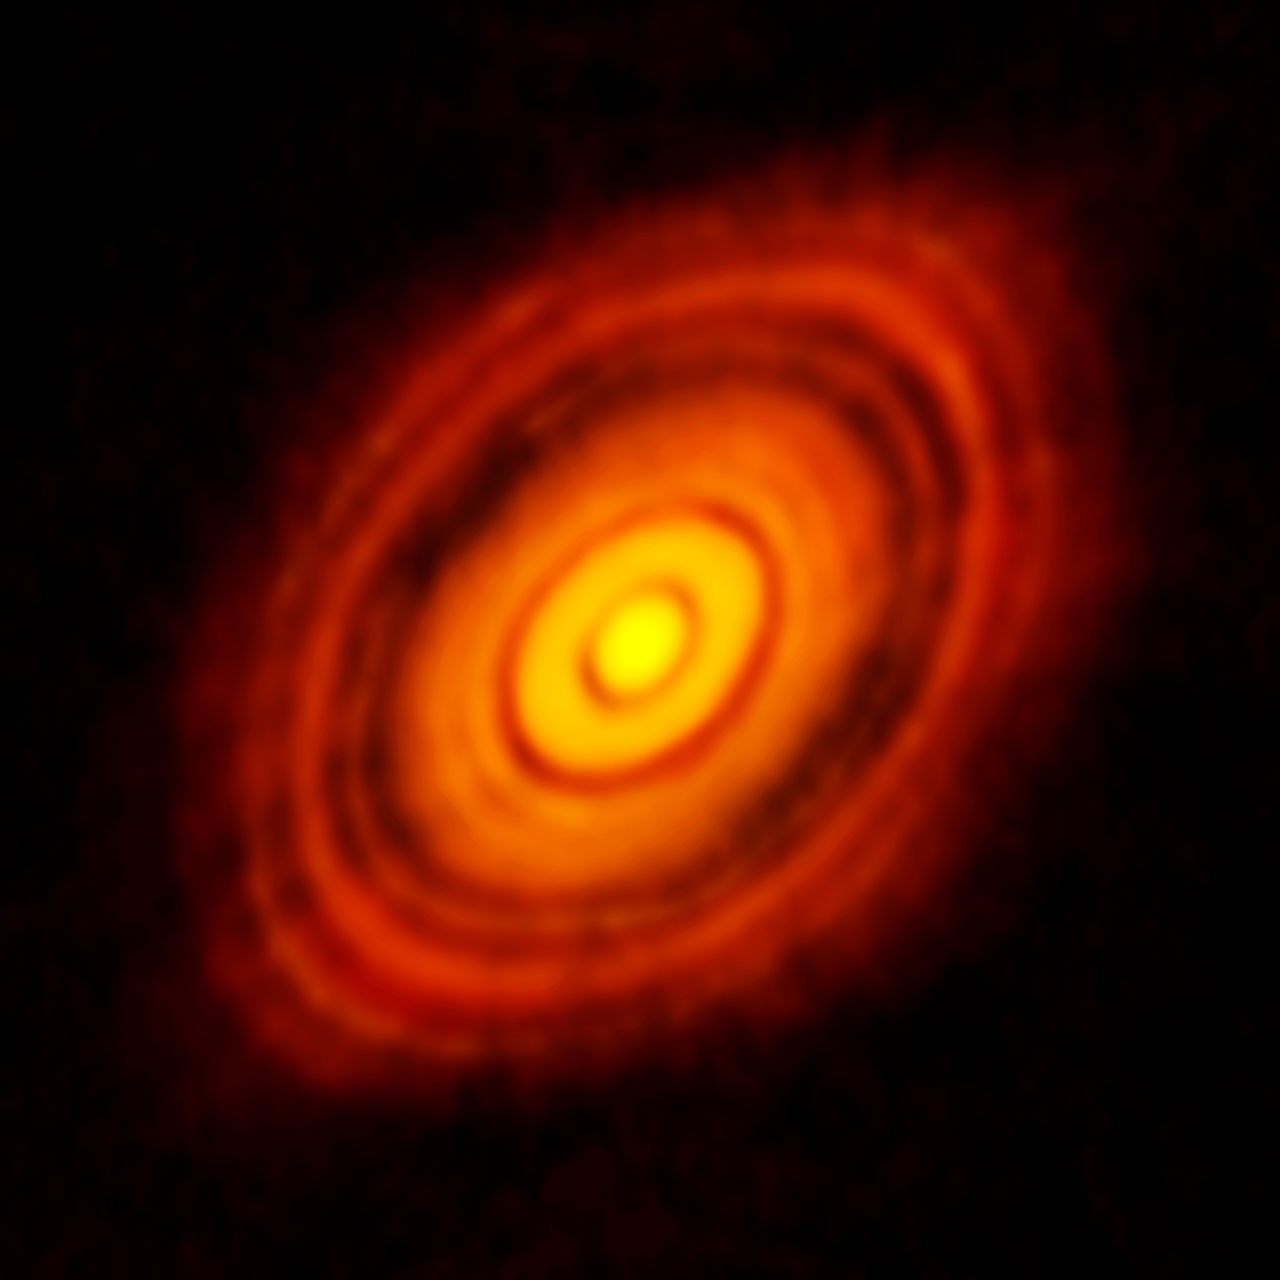
\includegraphics[scale=0.2]{HL_tau.jpg}
% \caption{\em{ALMA image of the protoplanetary disc surrounding the young star HL Tauri.}}
% \end{figure}
%-----------------------------Figure End------------------------------

%-----------------------------Table Start-----------------------------

% Minimum font size for references: 12pt 
% Proposals not compliant to this will be rejected. See Section 5.3.1 in the ALMA Proposer's Guide.

% \begin{table}[tbh]
% \begin{center}
% \caption[]{\em{Here we show the continuum sensitivity required per band.}}
% \begin{tabular}{cc}
% \hline \noalign {\smallskip}
% Frequency (GHz) & Sensitivity (mJy) \\
% \hline \noalign {\smallskip}
% 300 & 0.10 \\
% 850 & 0.50 \\
% \hline \noalign {\smallskip}
% \end{tabular}
% \end{center}
% \end{table}
%-----------------------------Table End ------------------------------

\section{Description of observations}

% Please describe the observations to be made and their specific
% purpose, with a clear explanation of the need for, and 
% appropriateness of, ALMA Cycle 9 data. 

\noindent \textbf{Spectral set-up} \quad We request to observe 6 \protonatedcarbondioxide lines in total using one Band 3 set-up and two Band 6 set-ups. The requested lines are summarized in Table \ref{tab:lines}. We selected the detectable lines with appropriate excitation energies and line strengths. In addition, we include several lines related to \carbondioxide sublimation, such as HCO$^+$ isotopologue, C$_2$H, and deuterated water (HDO) lines, which will be used to fully reveal the \carbondioxide sublimation region.


\begin{table}[tbh]
\vspace{-1em}
\begin{center}
\caption[]{\emph{Target lines and expected intensities}}
\begin{tabular}{cccccc}
\hline \hline \noalign {\smallskip}
Specie & Transition & $\nu_0$ [GHz] & $S\mu^2$ [D$^2$] & $E_\mathrm{up}$ [K] & Expected $I_\nu$ [mJy\,beam$^{-1}$] \\
\hline \noalign {\smallskip}
\multicolumn{6}{c}{Band 3 set-up} \\
\hline
\protonatedcarbondioxide & 4$_{0,4}$--3$_{0,3}$ & 85.532 & 16.0 & 10.3 & $\sim$13 \\
\protonatedcarbondioxide & 4$_{1,3}$--3$_{1,2}$ & 85.853 & 15.0 & 47.7 & $\sim$6.0 \\
\hline 
\multicolumn{6}{c}{Band 6 set-up 1} \\
\hline
\protonatedcarbondioxide & 10$_{0,10}$--9$_{0,9}$ & 213.813 & 40.0 & 56.4 & $\sim$35 \\
\protonatedcarbondioxide & 10$_{1,9}$--9$_{1,8}$ & 214.619 & 39.6 & 93.9 & $\sim$18 \\
\hline 
\multicolumn{6}{c}{Band 6 set-up 2} \\
\hline
\protonatedcarbondioxide & 12$_{1,12}$--11$_{1,11}$ & 255.564 & 47.7 & 117 & $\sim$23 \\
\protonatedcarbondioxide & 12$_{0,12}$--11$_{0,11}$ & 256.566 & 48.0 & 80.0 & $\sim$45 \\
\hline \noalign {\smallskip}
\end{tabular}
\label{tab:lines}
\end{center}
\vspace{-2em}
\end{table}

\noindent \textbf{Angular resolution and sensitivity} \quad Based on the dust temperature distribution derived from previous continuum observations \citep{Jacobsen19}, the expected location of the \carbondioxide snowline (where the temperature is $\sim$50\,K) is $\sim$180\,au in radius (or $\sim$360\,au in diameter, $\sim$1\farcs8), which corresponds to the outer edge of \protonatedcarbondioxide distribution. We request to spatially resolve the \carbondioxide sublimation region with a 0\farcs28 beam in Band 6 and a 0\farcs5 beam in Band 3 (or $\sim$60--100\,au in diameter). While the coarser Band 3 resolution reflects a compromise between resolving the \protonatedcarbondioxide emitting region and integration time, we pursue the higher angular resolution in Band 6. These resolutions also enable us to detect the expected inner cavity of \protonatedcarbondioxide associated with water sublimation. The size of the water sublimation region should be $\sim$0\farcs3--0\farcs5 (or $\sim$60--100\,au) in diameter based on the \water isotopologue observations \citep{Jensen19, Jensen21}. 

To evaluate the expected intensity of the target lines, we used the astrochemical model for prototypical protostellar envelopes based on the method presented in \citet[][, Figure \ref{fig:protocore_cartoon}(b)]{Aikawa20}, which reproduces the observed \protonatedcarbondioxide abundance in the outer cold envelope. The expected line intensities are summarized in Table \ref{tab:lines} when assuming the \protonatedcarbondioxide abundance at around 50--100\,K region in the model ($\sim2\times10^{-11}$) and an excitation temperature of $\sim$50\,K. We request sensitivities of 1.2 mJy per 0\farcs5 beam for Band 3 to detect target lines at $>5\sigma$, and 1.8 mJy per 0\farcs28 beam for Band 6 to detect at $>10\sigma$. We note that even if the target lines are not detected, we can put a strict upper limit on the \protonatedcarbondioxide and then \carbondioxide abundances, from which we will discuss the sublimation of \carbondioxide and provide important implications on the \carbondioxide chemistry. 



% The \protonatedcarbondioxide emission is expected to have a distribution with the inner cavity whose outer edge corresponds to the \ce{H2O} sublimation front. Based on the water and COMs observations (Oya et al. 2017; Jacobsen et al, 2019: Jensen et al. 2019), we expect the inner cavity with the size of $\sim$100\,au in diameter. In order to resolve the cavity, we set the spatial resolution to 0.5$''$ for Band 3 and 0.25$''$ for Band 6. We note that the \ce{CO2} sublimation front, which is our primary goal, is clearly resolved with the requested sensitivity since its location is expected to be further away from the central protostar.

% \par
% Based on the dust temperature distribution calculated by Jacobsen et al. (2019) (Figure 3) and the peak intensity of \protonatedcarbondioxide 4$_{0,4}$--3$_{0,3}$ line by Ag\'undez et al. (2019), we request the sensitivity of 1.5\,K for Band 3 setup and 2\,K and 1.75\,K for two Band 6 setups respectively. These sensitivities are adjusted for the weakest lines among each setup, i.e., \protonatedcarbondioxide 4$_{1,3}$-3$_{1,2}$ in Band 3,  \protonatedcarbondioxide 10$_{1,9}$--9$_{1,8}$ in Band 6 setup 1, and \protonatedcarbondioxide 12$_{1,12}$--11$_{1,11}$ in Band 6 setup 2, to be detected at 20$\sigma$, sufficient to achieve the all of the science goal. In the case of non-detection, we can constrain a strict upper limit on \protonatedcarbondioxide abundance, and finally \ce{CO2} abundance.


\vspace{-1em}
\section*{References}
\vspace{-0.5em}
\bibliographystyle{aas_compactbib}
\bibliography{reference}

% \section{References}

% List references here
% Minimum font size for references: 12pt 
% Proposals not compliant to this will be rejected. See Section 5.3.1 in the ALMA Proposer's Guide.

% \noindent [1] Author1 et al. year, journal, vol, page

% \noindent [2] Author2 et al. year, journal, vol, page


%%%%%%%%%%%%%%%%%%%%%%%%%%%
%%%%% End of document %%%%%
%%%%%%%%%%%%%%%%%%%%%%%%%%%

\end{document}

